\documentclass{jsarticle}
\usepackage{bm}
\usepackage{fancyhdr}
\usepackage{amsmath}
\usepackage{amssymb}
\usepackage{braket}
\usepackage{booktabs}
\usepackage{array}
\usepackage{graphicx}
\usepackage{here}
\usepackage{multicol}
\usepackage{okumacro}
\usepackage[dvipdfmx]{hyperref}
\usepackage{pxjahyper}
\usepackage{color}
\usepackage{ascmac}
\usepackage{url}
%\usepackage{txfonts}



%\pagestyle{empty}
\pagestyle{fancy}


\begin{document}

\title{EASIROC User's Guide}
%\author{}
\date{2019/5/9}
\maketitle


\newpage
\section{EASIROCについて}
Monolithic MPPC arrayは、高い集積度で検出器を作ることを可能にするが、大面積をカバーする場合多くのチャンネル数が必要となる。またブレイクダウン電圧や印加電圧とゲインの関係が単一の Monolithic MPPC array 上の MPPC 間でも異なるため、各 MPPC への印加電圧を調整する必要がある。この二つの要請を満たすために MPPC 読み出しシステムとして KEK 及び OpenIt が2013年に EASIROC ボード(GN-1101-1,GN-1101-2R) を開発した[1]。どちらのボードもファームウェアは EASIROC pro v4.4 を使用している。これは ASIC に OMEGA 社のEASIROC1 チップを用いた読み出しボードである。このチップの特性として主なものを以下に挙げる。
\begin{itemize}
\item 32チャンネル同時読み出し
\item 正電圧入力、Amp、shaping後、正電圧出力
\item 0 - 4.5 V、8 bit 程度のバイアス電圧調整機能
\item discriminator を内蔵
\item slow control でパラメータの調整が可能
\item 入力電荷として 160 fC から 320 pC までのダイナミックレンジをカバー(これはMPPC のゲインを$10^6$と仮定すると 1 p.e. - 2000 p.e. に相当)
\end{itemize}

その後、WAGASCI の MPPC mass test に使用できるように2015年に東京大学がアップグレードし[2]、Scaler や TDC 情報を取得できるように改良した。

\newpage
\section{EASIROCの内部動作}
ボードの内部には2つのEASIROCチップが埋まっており、最大で 64チャンネルの MPPC を同時に読み出すことができる。EASIROC チップからのアナログ信号は4つの ADC でデジタル信号に変換、Discriminator 出力は MHTDC 及び Scaler に入力され、Gatherer、Sender、SiTCP を介してデータ取得PC(DAC)に渡される。DAC と EASIROC ボード は Ethernet ケーブルでつながっている。必要な動作電圧は +6 V であり、NIMビンから供給可能である。
\begin{figure}[H]
\begin{center}
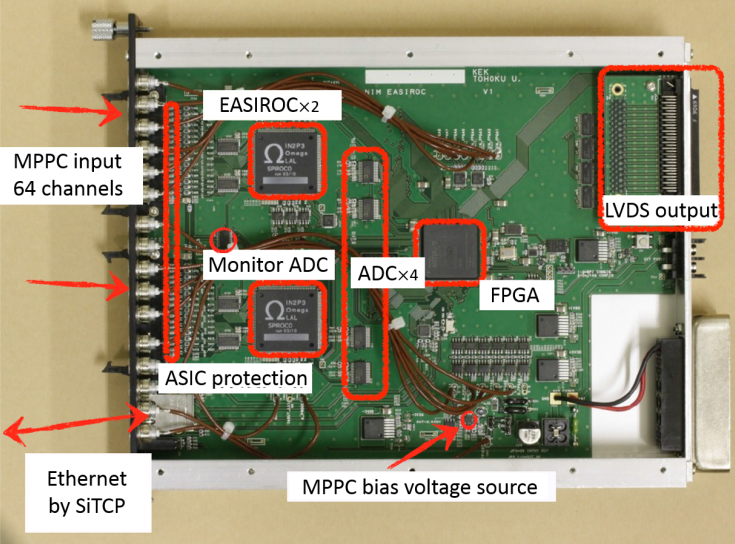
\includegraphics[width = 10.0cm, bb= 0 0 735 544]{2.png}
\end{center}
\caption{NIM-EASIROCボードの側面}
\label{fig:}
\end{figure}

\begin{figure}[H]
\begin{center}
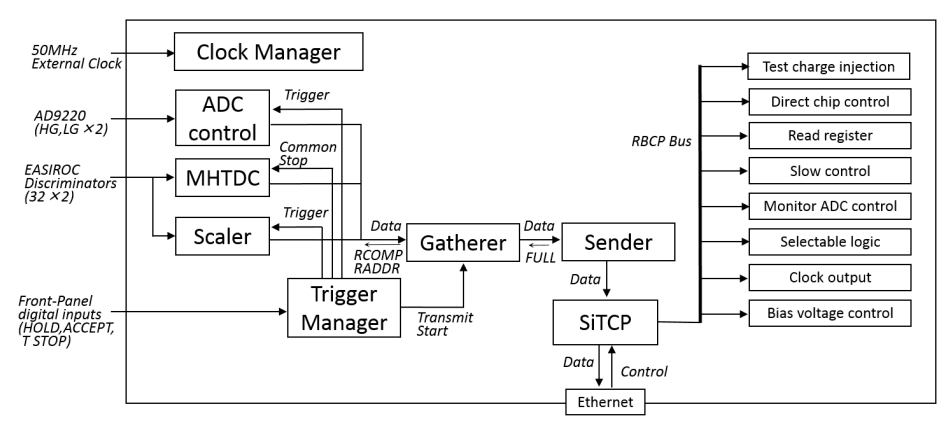
\includegraphics[width = 10.0cm, bb= 0 0 952 424]{3.png}
\end{center}
\caption{NIM-EASIROCボードの回路イメージ}
\label{fig:}
\end{figure}

\begin{figure}[H]
\begin{center}
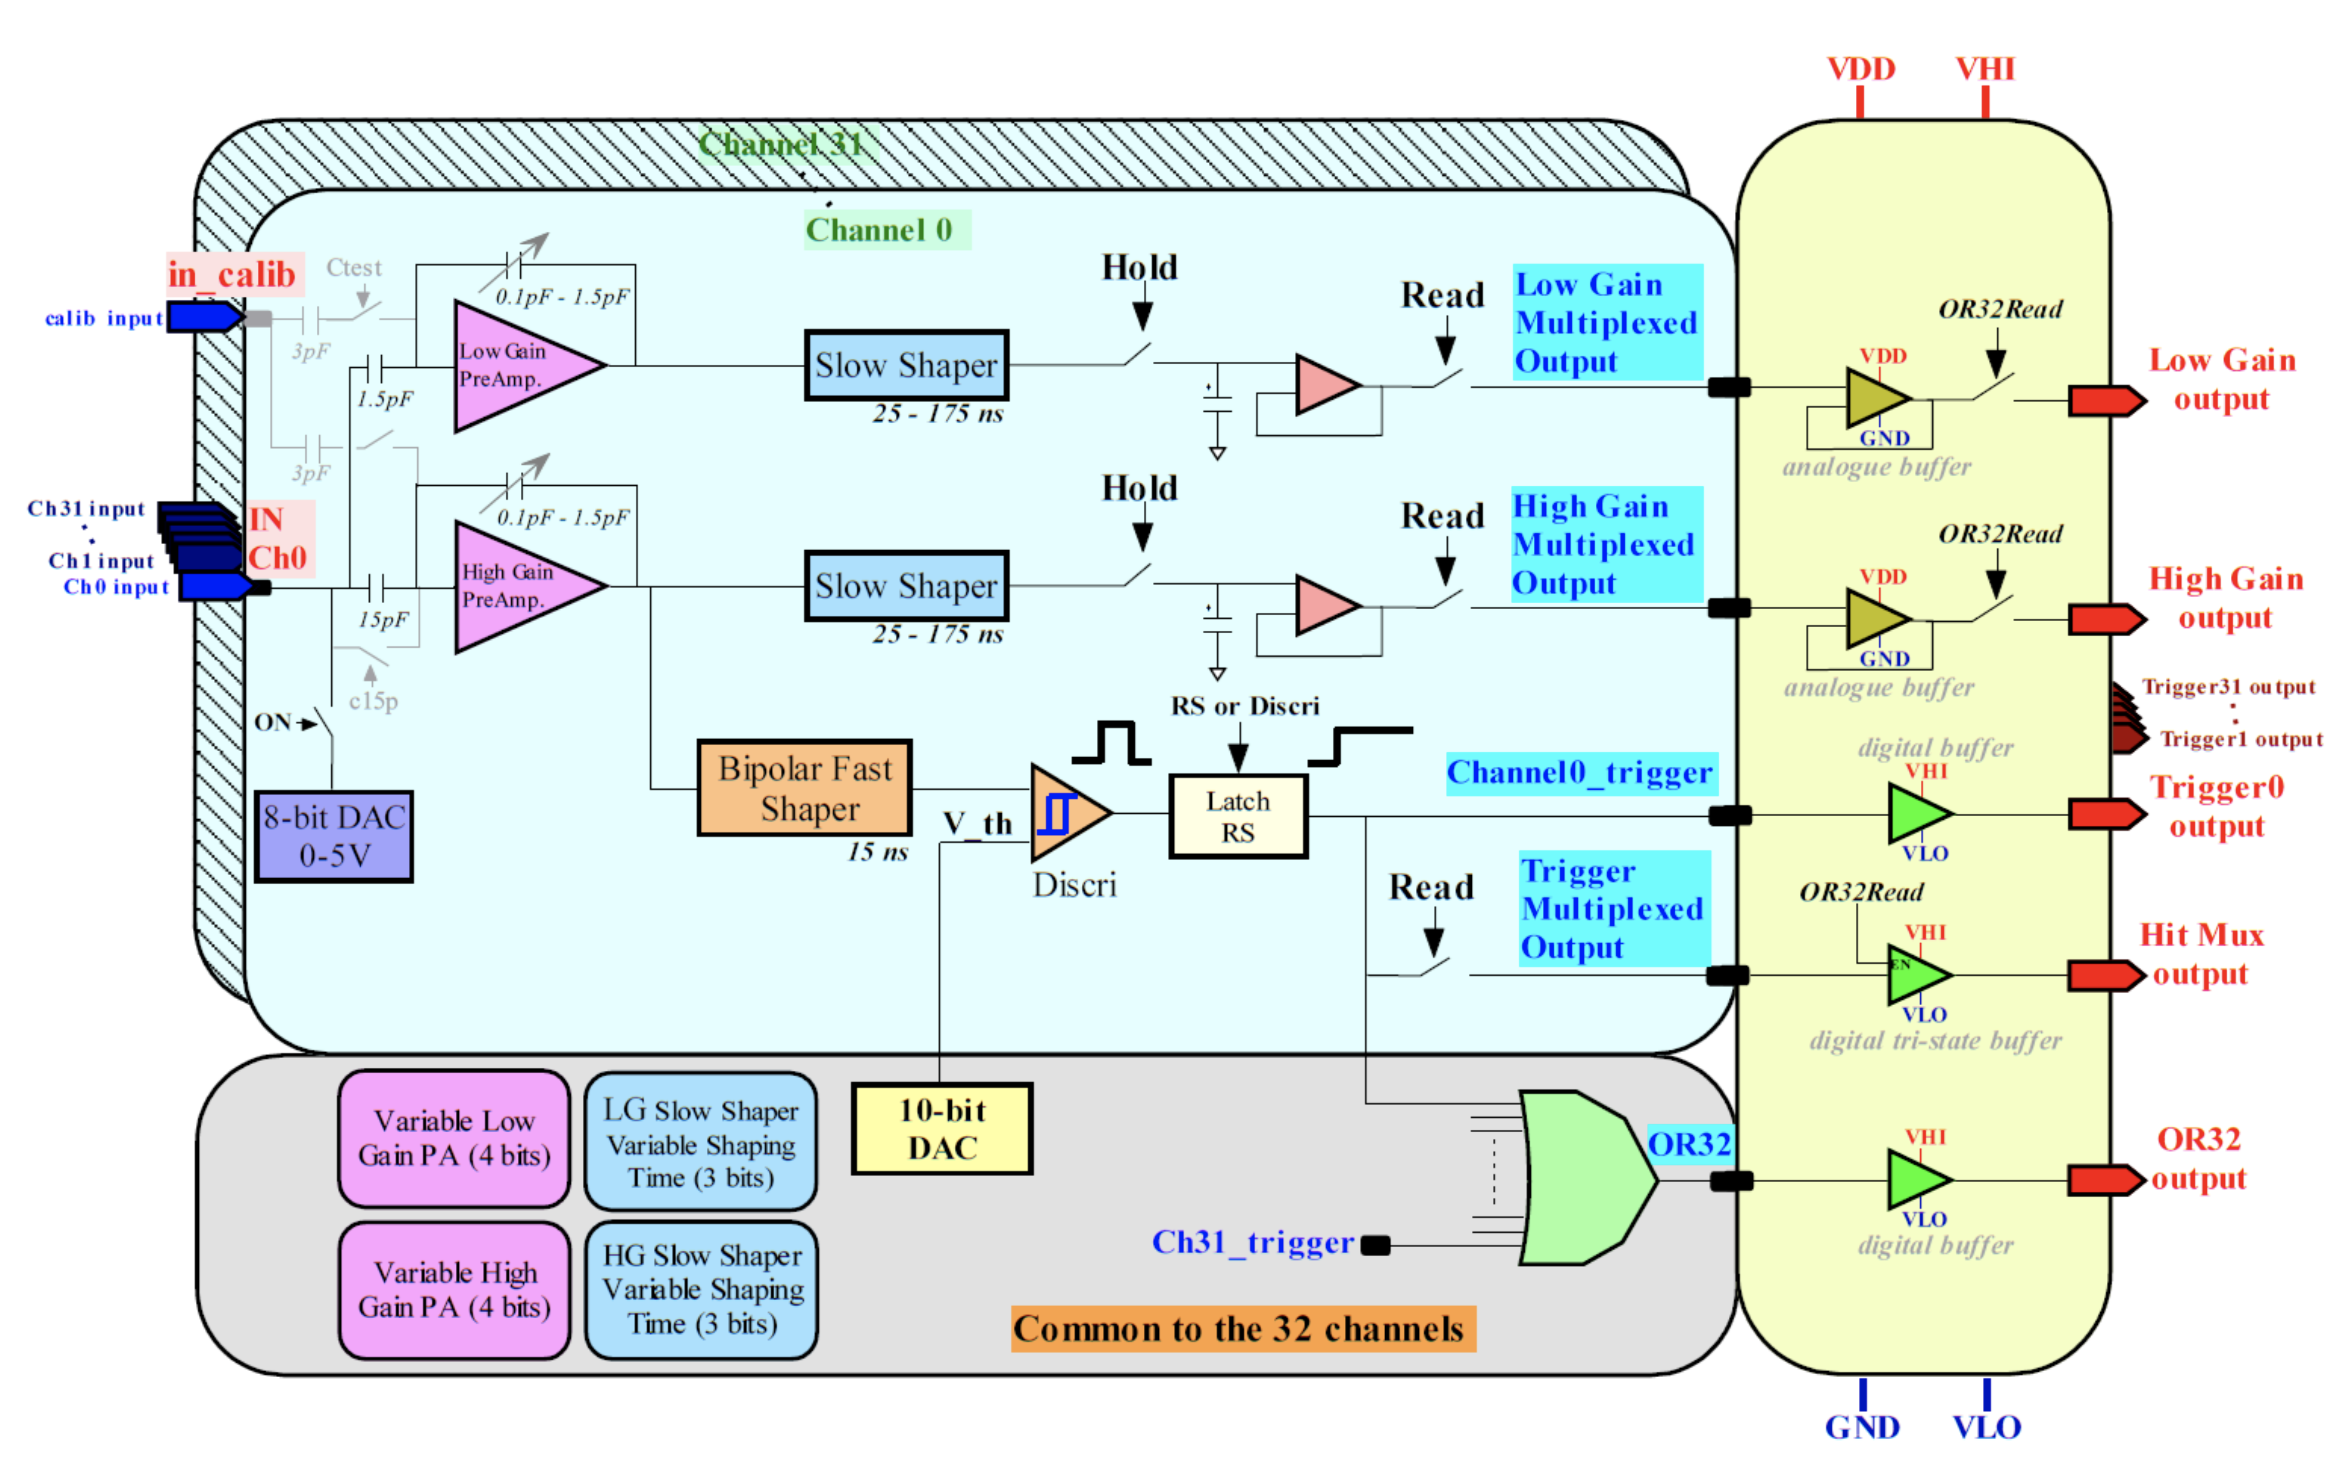
\includegraphics[width = 13.0cm, bb= 0 0 1167 735]{5.png}
\end{center}
\caption{EASIROC チップのブロックダイアグラム}
\label{fig:}
\end{figure}

アナログ信号の変換手順は以下のようになる。
\begin{enumerate}
\item Low 及び High 二つの異なるゲインを持つプリアンプにより電荷が積分・増幅される
\item プリアンプ出力は Fast shaper 及び Slow shaper に入力される
\item Fast shaper に入った信号は時定数 15 ns で整形され、Discriminator の Threshold を超えた場合にデジタル信号に変換される
\item Slow shaper に入った信号は時定数 25 - 175 ns で整形され、HOLD 信号を受け取った瞬間の電圧値が保持・記録される
\end{enumerate}


\newpage
\section{EASIROCの使い方}
\subsection{トリガー信号}
基本的に外部トリガーのみに対応している。内部トリガーを用いるには、出力 Triger 信号に適切な delay をかけて"HOLD", "T STOP", "ACCEPT" の順に入力する必要がある。

タイミングの制約として、HOLD - ACCEPT 間は大体 2 us 以上必要(ADC の変換レートによる)。2.5 us あれば確実。

\begin{figure}[H]
\begin{center}
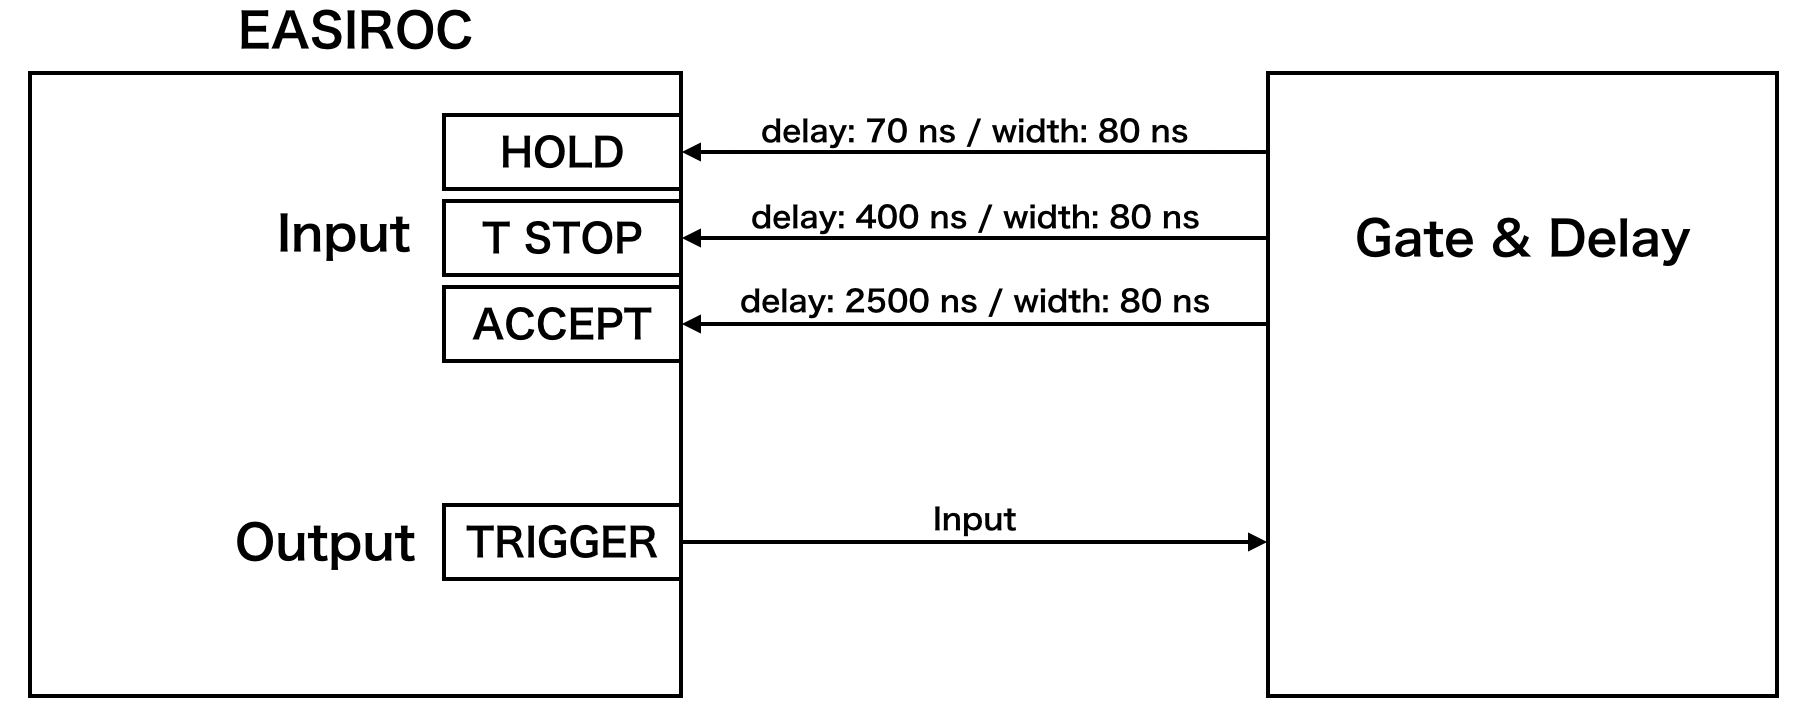
\includegraphics[width = 13.0cm, bb= 0 0 899 358]{1.png}
\end{center}
\caption{内部トリガー信号回路の一例[1]}
\label{fig:}
\end{figure}

\begin{figure}[H]
\begin{center}
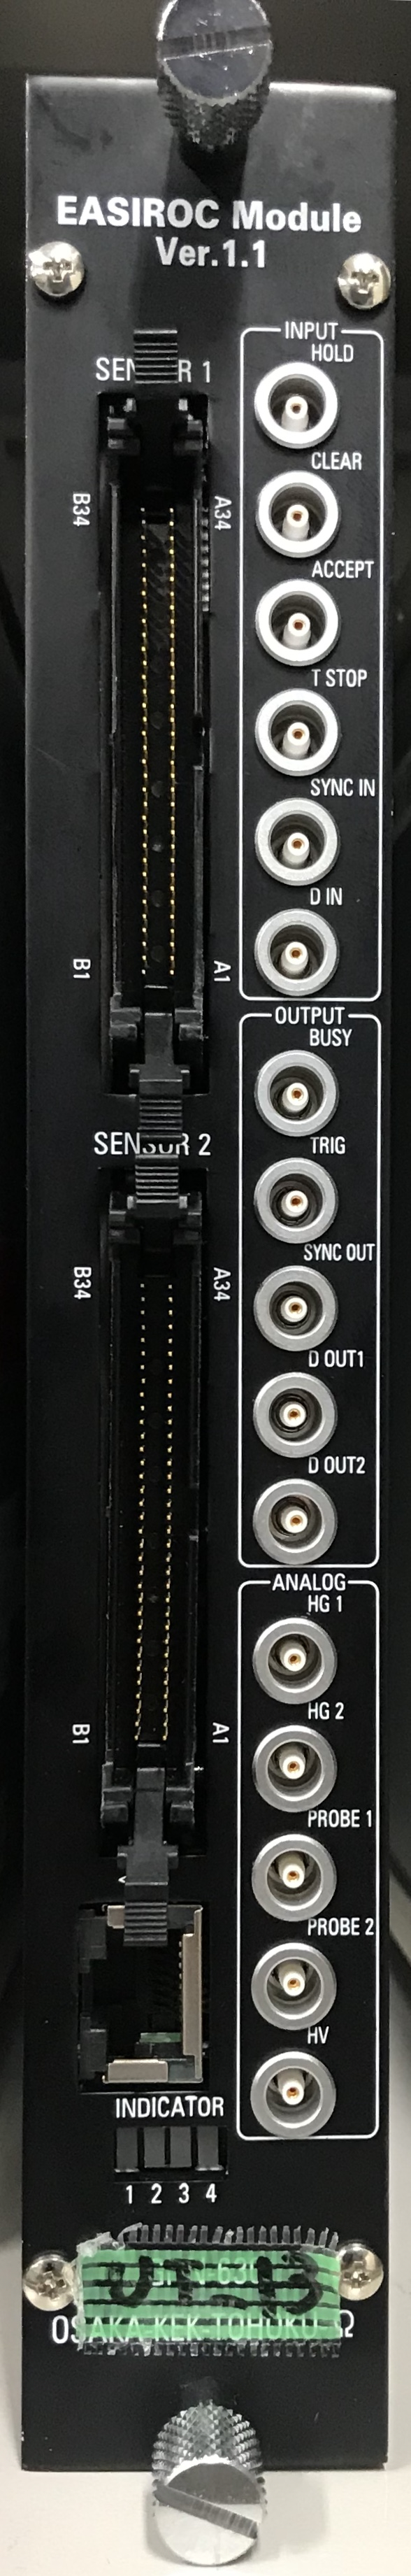
\includegraphics[width = 1.3cm, bb= 0 0 588 3683]{4.jpg}
\end{center}
\caption{EASIROC ボードのフロントパネル}
\label{fig:}
\end{figure}

\newpage
\subsection{対話モード}
内部で Readline が動いており、対話的に EASIROC を操作できる。
\subsubsection{対話モード}
EASIROC対話モードの起動
\begin{shadebox}
\begin{verbatim}
$ ./Controller.rb [IP Address (default: 192.168.10.16)]
\end{verbatim}
\end{shadebox}
 \\
EASIROC対話モードの終了
\begin{shadebox}
\begin{verbatim}
> exit [quit]
\end{verbatim}
\end{shadebox}


\subsubsection{バイアス電圧の設定}

HVの電圧と電流値を表示する
\begin{shadebox}
\begin{verbatim}
> statusHV
\end{verbatim}
\end{shadebox}
 \\
HVを[bias voltage]の値に設定する
\begin{shadebox}
\begin{verbatim}
> setHV [bias voltage]
\end{verbatim}
\end{shadebox}
 \\
HVを[bias voltage]の値まで複数回のstepで上昇。各stepで電流値を確認しリミットに到達したらstopする。
\begin{shadebox}
\begin{verbatim}
> increaseHV [bias voltage]
\end{verbatim}
\end{shadebox}

\subsubsection{データ取得に関わる操作}
Slow controllの値を反映する
\begin{shadebox}
\begin{verbatim}
> slowcontrol
\end{verbatim}
\end{shadebox}
 \\
データ取得を行う
\begin{shadebox}
\begin{verbatim}
> read [Event #] [Filename]
\end{verbatim}
\end{shadebox}
 \\
ADC [TDC/Scaler] をON/OFFにする
\begin{shadebox}
\begin{verbatim}
> adc [on/off]
> tdc [on/off]
> scaler [on/off]
\end{verbatim}
\end{shadebox}
使わないときはOFFにすることでデータ取得が高速になる。

\subsubsection{諸々の情報}
\begin{itemize}
\item 対話時に入力されたコマンドは CommandDispatcher クラスによって処理される
\item 対話モードでhelp と入力してヘルプが見られる
\item 各コマンドは変数 COMMANDS に含まれているものが利用可能で、それぞれのコマンドはメソッドによって処理される
\item シェルのコマンドも一部使えるようになっている(ex. ls, mv, root)
\item それらは変数 DIRECT\_COMMANDS に含まれているものが利用可能
\item Controller ディレクトリ内で hist.cc を make してプログラムを生成していれば、read 終了後に自動でヒストグラムを生成する。出力先は Controller/data ディレクトリ内。
\end{itemize}

\newpage
\subsection{Slow Controll}
Slow Controll は yaml ディレクトリ下の YAML ファイル(拡張子:yml)によって指定される。\\
YAML は構造化されたデータを表現するフォーマットで、XML と似ているが YAML の方が人間にとって理解しやすい形式になっている。よく使いそうなものを以下に紹介する。

\subsubsection{RegisterValue.yml}

\begin{shadebox}
\begin{verbatim}
EASIROC1:  # チップごとに設定
         Capacitor HG PA Fdbck: 100fF    # 増幅率を決定。キャパシタの値は
         Capacitor LG PA Fdbck: 100fF    # RegisterValueAlias.yml に含まれる。
         Time Constant HG Shaper: 100ns  # SlowShaper の時定数
         Time Constant LG Shaper: 50ns
         DAC code: 600  # FastShaper 後段の Discriminator の閾値
 
EASIROC2:
         Capacitor HG PA Fdbck: same
         Capacitor LG PA Fdbck: same
         Time Constant HG Shaper: same
         Time Constant LG Shaper: same
         DAC code: same
 
High Gain Channel 1: 0   # HG1/HG2 で読み出すチャンネルの指定。
High Gain Channel 2: -1  # 読み出すなら0、読み出さないなら-1。
Probe Channel 1: -1      # フロントパネルの Probe からの出力チャンネル選択
Probe Channel 2: -1
Probe 1: Out_fs
Probe 2: Out_fs  # Out_PA_HG, Out_PA_LG, Out_ssh_HG, Out_ssh_LG, Out_fs
SelectableLogic:
         Pattern: Or64        # OneCh_#, Or32u, Or32d, Or64, Or32And,...
         HitNum Threshold: 4  # Threshold for each OR logic. 0~64. Default: 0
         And Channels: -1     # Cannels used in And Logic. 0~63. Default: -1
TimeWindow: 4095ns
UsrClkOut: "OFF"  # フロントパネルの syn out から出力される周期信号 # "ON", 1Hz,...
Trigger:          ## This "Trigger" values are not used for this version.
         Mode: 0  #0-7
         DelayTrigger: -1   #500MHz #default:-1, 0-253 #trig -> hold -> l1 -> l2
         DelayHold: -1      #25MHz
         DelayL1Trig: -1    #6MHz
         Width: raw
\end{verbatim}
\end{shadebox}
Discriminator の DAC 値を大きくするとThreshold は下がる。

\subsubsection{InputDAC.yml}
8-bit Input DACの値がチップごとに32ch分並んでいる。256 - 511 で調整(最上位ビットはenableのため常に1)。\\
DAC 値を上げるとバイアス電圧は小さくなる。
\begin{shadebox}
\begin{verbatim}
---
EASIROC1:
  Input 8-bit DAC:
  - 350
  - 350
  - 350
  - 350
  - 350
  - 350
  - 350
  - 350
\end{verbatim}
\end{shadebox}

\subsubsection{Calibration.yml}

\begin{shadebox}
\begin{verbatim}
HVControl:   # 指定した HV を DAC 値に変換する係数
        - 413.9 #423.06 #483.183
        - 747.8 #767.17 #780.0
MonitorADC:  # Monitor ADC で読み取った値を電圧、電流、温度に変換する係数
        HV: 0.00208 #0.3235 #0.00208
        HVOffset: 0.0355 #4.1694
        Current: 0.0364 #0.034
        InputDac: 0.00006866 #4.5/2^16 #0.0000685
        Temperature: 4500.0
\end{verbatim}
\end{shadebox}

\newpage
\subsection{その他}

\subsubsection{Probe 出力}


\begin{multicols}{2}
信号処理中の中間信号を取り出すための Probe 出力ラインがフロントパネルに用意されている。出力することができる中間信号を以下に示す。
\begin{itemize}
\item HighGain PreAmp 出力
\item LowGain PreAmp 出力
\item HighGain Slow shaper 出力
\item LowGain Slow shaper 出力
\item Fast shaper
\end{itemize}
前述の RegisterValue.yml から出力する情報を指定することができる。\\

PreAmp を選択した場合、波形全体ではなくピーク付近の一部のみ出力される。注意点としては、2 ch 以上を同時に ON にしない、データ取得中は Probe 1,2 を OFF にすること。


\begin{figure}[H]
\begin{center}
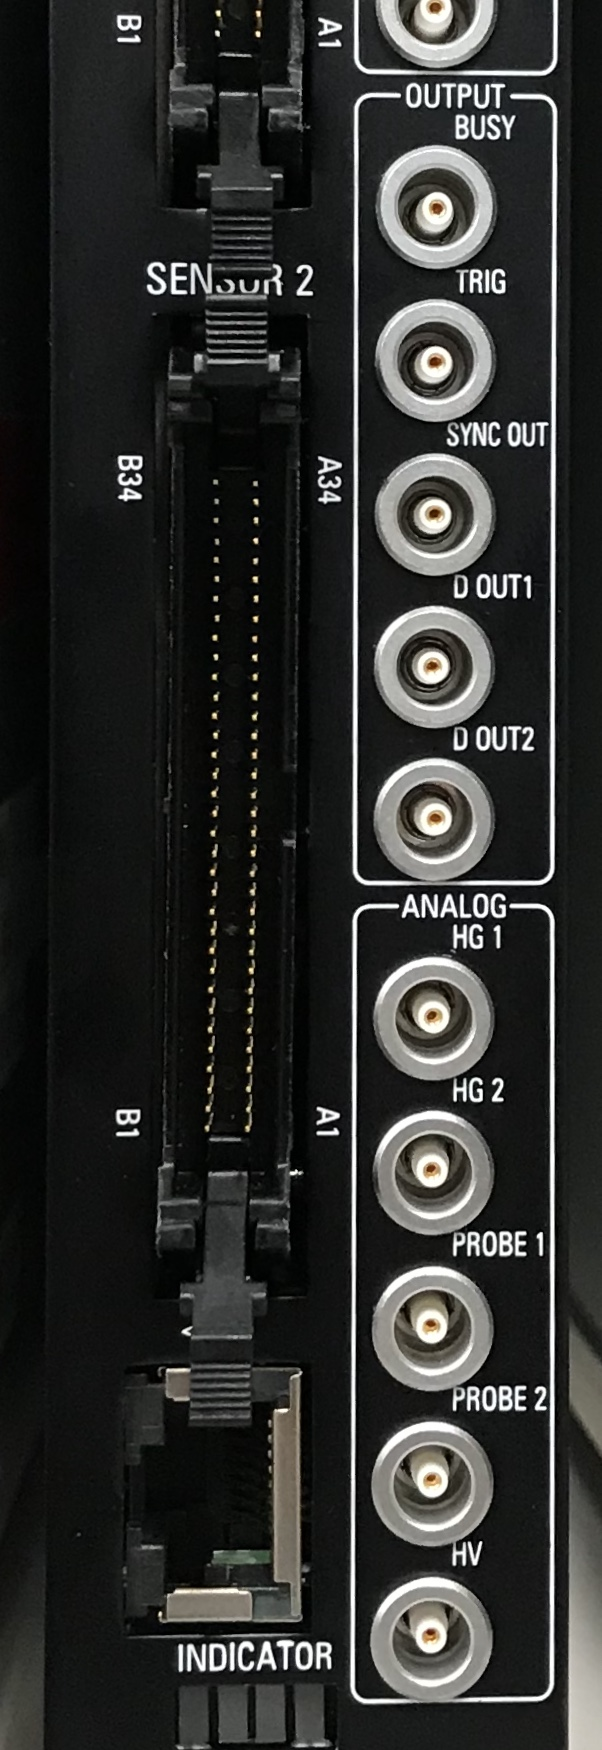
\includegraphics[width = 3cm, bb= 0 0 602 1750]{6.jpg}
\end{center}
\caption{フロントパネルの Probe 出力}
\label{fig:}
\end{figure}
\end{multicols}


\begin{shadebox}
\begin{verbatim}
High Gain Channel 1: 0   # HG で読み出すチャンネルの指定
High Gain Channel 2: -1  # 読み出すなら ch_#、読み出さないなら-1
Probe Channel 1: -1      # Probe からの出力チャンネル選択
Probe Channel 2: -1      # 2 ch 以上同時に使用しない
Probe 1: Out_PA_HG
Probe 2: Out_fs  # Out_PA_HG, Out_PA_LG, Out_ssh_HG, Out_ssh_LG, Out_fs
\end{verbatim}
\end{shadebox}
 \\
また、SYNC OUT からの周期信号も RegisterValue.yml より変更が可能である。

\begin{shadebox}
\begin{verbatim}
UsrClkOut: "OFF"  # "OFF", "ON", 1Hz, 10Hz, 100Hz, 1kHz, 10kHz, 100kHz, 3MHz, ...
\end{verbatim}
\end{shadebox}


\newpage
\subsubsection{横山研所有のEASIROC}
2019年5月9日現在、5つの EASIROC ボードの存在が確認された。うち一つは京大高エネルギー研究室の備品と思われる。IP アドレスは DAC との接続の際に必要となる。
\begin{table}[H]
\begin{center}
\caption{横山研所有のEASIROC}
\begin{tabular}{ccc} \hline
管理No. & IP Adress & 備考 \\ \hline
1 & 192.168.10.11 &  \\ 
2 & 192.168.10.12 &  \\ 
3 & 192.168.10.13 &  \\ 
2号 & 192.168.10.18 & ch.32 の読み出し不調。バイアス HV にふらつきあり。 \\ 
京大高エネ備品 & 不明 & 後半 32ch の InputDAC が動かない。連絡先:075-753-3837。  \\ \hline
\end{tabular}
\end{center}
\end{table}


\newpage
\section{参考文献}
1,2,3 は EASIROC 開発時の資料、4,5 はアップグレード後の資料である。
\begin{enumerate}
\item OpenIt のサイト\\
\url{http://openit.kek.jp/project/MPPC-Readout-Module/public/MPPC-Readout-Module}
\item 石島さんの修論\\
\url{http://osksn2.hep.sci.osaka-u.ac.jp/theses/master/2013/ishijima_mthesis.pdf}
\item 塩崎さんの修論\\
\url{http://lambda.phys.tohoku.ac.jp/~db/human_resource/thesis/2009_B_2_M_1.pdf}
\item 竹馬さんのマニュアル\\
\url{http://hep.phys.s.u-tokyo.ac.jp/~nchikuma/easiroc_manual.html} 
\item 竹馬さんの修論\\
\url{http://hep.phys.s.u-tokyo.ac.jp/wordpress/wp-content/uploads/2016/06/mth2016_chikuma.pdf}
\end{enumerate}

\end{document}
%%%%%%%%%%%%%%%%%%%%%%%%%%%%%%%%%%%
%%%%%%%%%%%%%%%%%%%%%%%%%%%%%%%%%%%
%%%%%%%%%%%%%%%%%%%%%%%%%%%%%%%%%%%
%%%%%%%%%%%%%%%%%%%%%%%%%%%%%%%%%%%
%%%%%%%%%%%%%%%%%%%%%%%%%%%%%%%%%%%





%%%%%%%%%%%%%%%%%%%%%%%%%%%%%%%%%%%
%%%%%%%%%%%%%%%%%%%%%%%%%%%%%%%%%%%
%%%%%%%%%%%%%%%%%%%%%%%%%%%%%%%%%%%

%表の挿入
\begin{table}[H]
\begin{center}
\caption{表のタイトル}
\begin{tabular}{ccc} \hline
 &  &  \\ \hline
 &  &  \\ 
 &  &  \\ 
 &  &  \\ 
 &  &  \\ \hline
\end{tabular}
\end{center}
\end{table}


%図の挿入
\begin{figure}[H]
\begin{center}
\includegraphics[width = 12.0cm, bb= 0 0 360 252]{ファイル名.eps}
\end{center}
\caption{グラフのタイトル}
\label{fig:}
\end{figure}


%図を2つ並列
\begin{figure}[H]
\begin{minipage}{0.50\hsize}
\begin{center}
\includegraphics[width = 4.0cm,bb=0 0 600 600]{.ps}
\end{center}
\caption{タイトル}
\label{fig:}
\end{minipage}
\begin{minipage}{0.50\hsize}
\begin{center}
\includegraphics[width = 4.0cm,bb=0 0 600 600]{.ps}
\end{center}
\caption{タイトル}
\label{fig:}
\end{minipage}
\end{figure}



%図を3つ並列
\begin{figure}[H]
\begin{minipage}{0.33\hsize}
\begin{center}
\includegraphics[width = 4.0cm,bb=0 0 600 600]{.ps}
\end{center}
\caption{タイトル}
\label{fig:}
\end{minipage}
\begin{minipage}{0.33\hsize}
\begin{center}
\includegraphics[width = 4.0cm,bb=0 0 600 600]{.ps}
\end{center}
\caption{タイトル}
\label{fig:}
\end{minipage}
\begin{minipage}{0.33\hsize}
\begin{center}
\includegraphics[width = 4.0cm,bb=0 0 600 600]{.ps}
\end{center}
\caption{タイトル}
\label{fig:}
\end{minipage}
\end{figure}


%文章と図の2段組
\begin{multicols}{2}
文章

\begin{figure}[H]
\begin{center}
\includegraphics[width = 7.0cm,bb=0 0 800 600]{.pdf}%図
\end{center}
\caption{タイトル}
\label{fig:1.1.1}
\end{figure}
\end{multicols}

\makeatletter

%----- Equation num brackets -------------------

\newcommand\eqnobrck[1]{[#1]}

%---- Test if a file is loaded ------------------

\newcommand\@iffileloaded[2]{%
    \expandafter\ifx\csname ver@#1.#2\endcsname\relax
       \expandafter\@secondoftwo
    \else
       \expandafter\@firstoftwo
    \fi}

%----- For right equation numbers --------------

\renewcommand\@eqnnum{{%
    \normalfont \normalcolor \eqnobrck{\theequation}}}

%---- For left equation numbers ----------------

\@iffileloaded{leqno}{clo}{%
    \renewcommand\@eqnnum{\hb@xt@.01\p@{}%
       \rlap{\normalfont\normalcolor
       \hskip -\displaywidth\eqnobrck{\theequation}}}
    }{}

%---- If amsmath is loaded ----------------------

\@ifpackageloaded{amsmath}{%
     \renewcommand\tagform@[1]{%
        \maketag@@@{\eqnobrck{\ignorespaces#1\unskip\@@italiccorr}}}
        }{}


 \renewcommand{\theequation}{%
   \thesection.\arabic{equation}}
  \@addtoreset{equation}{section}


\makeatother




